%%%%% Description: beamer overlay for history of (weak) consistency models in the context of distributed systems. %%%%%
%%%%% Date: July 25, 2016 %%%%%
%%%%% Author: Hengfeng Wei (hengxin) %%%%

\begin{tikzpicture}[comment/.style = {align = center},
	axis/.style = {dashed, dash pattern = on 8pt off 4pt, line width = 2pt, draw = red},
	sepline/.style = {dashed, line width = 2pt, opacity = 0.80, blue},
    node distance = 2.0cm]

  %%%%%%%%%% Begin: years and papers %%%%%%%%%% 
  % \x: x coordinate; \y: year; \n: name; \lbl: label
  \foreach \x/\y/\n/\lbl in {
	1/1995/eventual/\textcolor{blue}{Eventual consistency},
	6/2000/cap/\textcolor{red}{\bf CAP theorem},
	12/2006/bigtable/\textcolor{blue}{Bigtable@Google},
	18/2007/dynamo/\textcolor{blue}{Dynamo@Amazon},
	25/2012/pacelc/\textcolor{red}{\bf PACELC tradeoff}} {
	\node[star, star points = 5, minimum size = 3pt, draw = red, fill = yellow, line width = 2pt] (\x) at (\x, 5) {};
	\node[below = 0.50cm of \x, font = \large] (\y) {\bf \y};
	\node[above = 0.50cm of \x, align = center, font = \Large] (\n) {\lbl};
  }

  \path[axis] (1) to (6) to (12) to (18) to (25);
  \draw[> = stealth, ->, axis] (25) to (27, 5);
  %%%%%%%%%% End: decades and systems %%%%%%%%%% 
  \draw[sepline] (8, 1) to (8, 10);
  \draw[sepline] (22, 1) to (22, 10);

  \pause
  %%%%% bayou system %%%%%
  \node[below = of 1995] (bayou-fig) {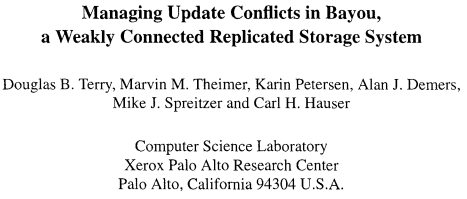
\includegraphics[scale = 0.35]{figs/bayou-paper.png}};
  \node[above = of eventual] (bayou-eventual) {
\includegraphics[scale = 0.13]{figs/24-7-service.png}};

  %%%%% cap theorem %%%%%
  \node[below = of 2000] (cap-ppt) {
\includegraphics[scale = 0.35]{figs/cap-keynote-ppt.png}};
  % \node[above = of cap] (cap-fig) {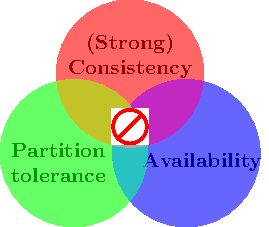
\includegraphics[scale = 0.90]{cap-theorem.pdf}}; 
  \node[above = of cap] (cap-fig) {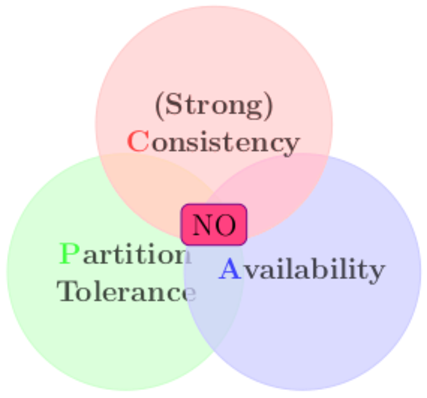
\includegraphics[scale = 0.55]{figs/cap-theorem-no-text.pdf}}; 

  \pause
  %%%%% bigtable %%%%%
  \node[below = of 2006, opacity = 0.80] (bigtable-fig) {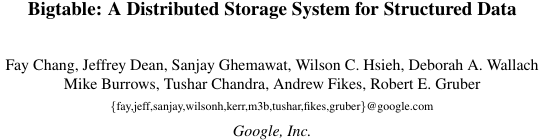
\includegraphics[scale = 0.50]{figs/bigtable-paper.png}};
  \node[above = of bigtable] (bigtable-tradeoff) {
\includegraphics[scale = 0.10]{figs/unavailable.png}};
  
  \pause
  %%%%% dynamo %%%%%
  \node[below = of 2007, opacity = 0.70] (dynamo-fig) {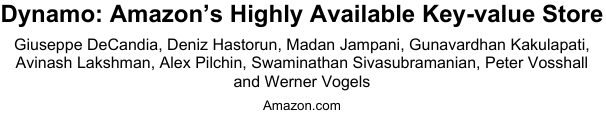
\includegraphics[scale = 0.50]{figs/dynamo-paper.png}};
  \node[above = of dynamo] (dynamo-tradeoff) {
\includegraphics[scale = 0.06]{figs/eventually.jpg}};

  \pause
  %%%%% more systems %%%%%
  \node[] (systems) at ($0.50*(bigtable) + 0.50*(dynamo) + (0, -0.50cm)$) {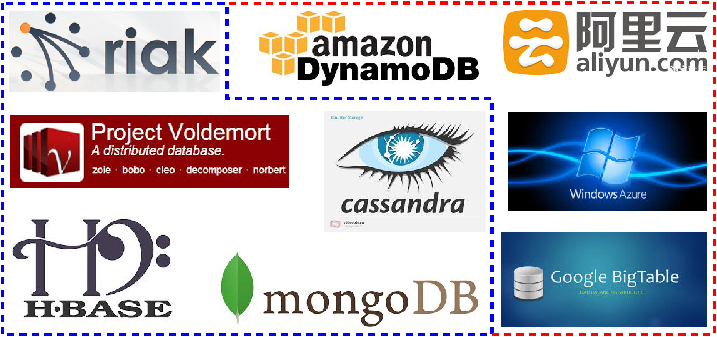
\includegraphics[scale = 0.80]{figs/dsss.pdf}};

  \pause
  %%%%% pacelc tradeoff %%%%%
  \node[below = of 2012] (pacelc-paper) {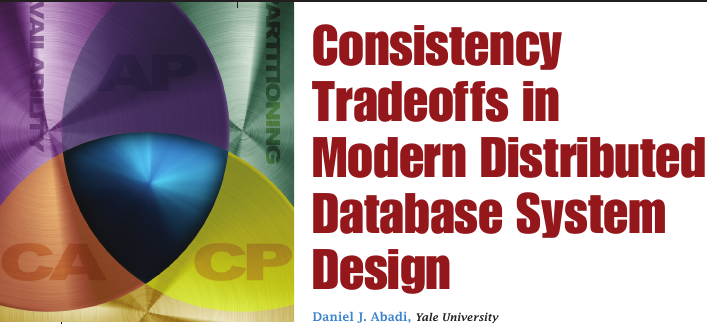
\includegraphics[scale = 0.25]{figs/pacelc-paper.png}};
  \node[above = of pacelc] (pacelc-fig) {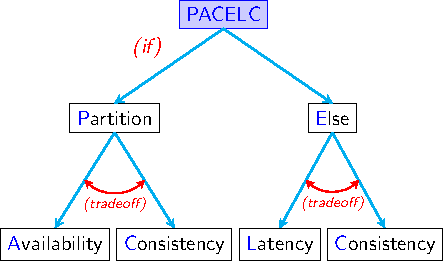
\includegraphics[scale = 0.80]{figs/pacelc-tradeoff-new.pdf}};
\end{tikzpicture}
